\documentclass[pdftex,12pt,a4paper]{article}

% --------------------------------------------- Imports  ----------------------------------------------

% Use auto command spaces formating 
\usepackage{xspace}
% Use spelling correction
\usepackage[german]{babel}
% Use graphics output format
\usepackage[pdftex]{graphicx}
% Use macros for adjusting boxed content
\usepackage{adjustbox}
% Use caption text format for images
\usepackage{caption}
% Use sub-caption text format for images
\usepackage{subcaption}
% Use listings for text enumerations
\usepackage{listings}
% Use colorful text for highlighting
\usepackage[usenames,dvipsnames]{color}
% Use hyphenate spacing, underlining, etc.
\usepackage{soul}
% Use header and footer
\usepackage[automark,headsepline]{scrpage2}
% Use URL formatting
\usepackage{url}
% Use mathematical formulas
\usepackage{amsmath,amssymb,amstext}
% Use different font formats
\usepackage{pxfonts}
% Use placement options
\usepackage{placeins}
% Use correct type of characters
\usepackage[T1]{fontenc}
\usepackage{booktabs}
\usepackage[table,xcdraw]{xcolor}
% Use pdf include package
\usepackage{pdfpages}
% Use color for formatting
\usepackage{color}
% Use page geometry
\usepackage[a4paper, total={6in, 8.5in}]{geometry}
% User utf8 characters
\usepackage[utf8]{inputenc}

% ------------------------------------------- Commands ---------------------------------------------

% Definitions for words to auto-complete
\newcommand{\sync}{synchrocyclotrons\xspace}
% Header format definition
\newcommand{\HRule}{\rule{\linewidth}{0.5mm}}

% Set document info templates
\newcommand{\UniversityName}{FH Hagenberg}

\newcommand{\AuthorFirstName}{Marius-Constantin}
\newcommand{\AuthorLastName}{Dinu}
\newcommand{\AuthorFullName}{\AuthorFirstName \xspace \AuthorLastName}
\newcommand{\MatrNr}{S1310307054}
\newcommand{\AuthorFirstNameCo}{Florian}
\newcommand{\AuthorLastNameCo}{Wurm}
\newcommand{\AuthorFullNameCo}{\AuthorFirstNameCo \xspace \AuthorLastNameCo}
\newcommand{\MatrNrCo}{S1310307112}
\newcommand{\AuthorFullID}{\AuthorFirstName \xspace \AuthorLastName \xspace (\MatrNr) \\ \AuthorFirstNameCo \xspace \AuthorLastNameCo \xspace (\MatrNrCo)}

\newcommand{\SubjectTitle}{SWK5 UEG2 SEv WS15/16}
\newcommand{\ExerciseTitle}{Ausbaustufe 1}

% Set document command shortcuts
\newcommand{\nPar}{\par\vspace{0.5cm}}
\newcommand{\nLine}{\par\vspace{0.1cm}}

% Set in-line highlighting
\newcommand{\code}{\texttt}

% ------------------------------------------- Formatting ---------------------------------------------

% Set document info
\title{\SubjectTitle \xspace \ExerciseTitle}
\author{\AuthorFullID}

% Set document header and footer
\pagestyle{scrheadings}
\clearscrheadfoot
\ihead[]{\SubjectTitle}
\ohead{\leftmark}
\cfoot[]{\pagemark}

% Disable indent globally
\setlength{\parindent}{0pt}

% Set syntax highlighting
\definecolor{mygray}{rgb}{0.4,0.4,0.4}
\definecolor{mygreen}{rgb}{0,0.7,0.5}
\definecolor{myorange}{rgb}{1.0,0.4,0}

% Set programming language style
\lstset{
    language=C++,
    basicstyle=\scriptsize\sffamily\color{black},
    commentstyle=\color{mygray},
    frame=single,
    breaklines=true,
    postbreak=\raisebox{0ex}[0ex][0ex]{\ensuremath{\color{red}\hookrightarrow\space}},
    numbers=left,
    linewidth=15cm,
    numbersep=5pt,
    numberstyle=\tiny\color{mygray},
    keywordstyle=\color{mygreen},
    showspaces=false,
    showstringspaces=false,
    stringstyle=\color{myorange},
    tabsize=2
}

% -------------------------------------------- Document ---------------------------------------------

\begin{document}

		\maketitle
		\newpage
		\tableofcontents
		
    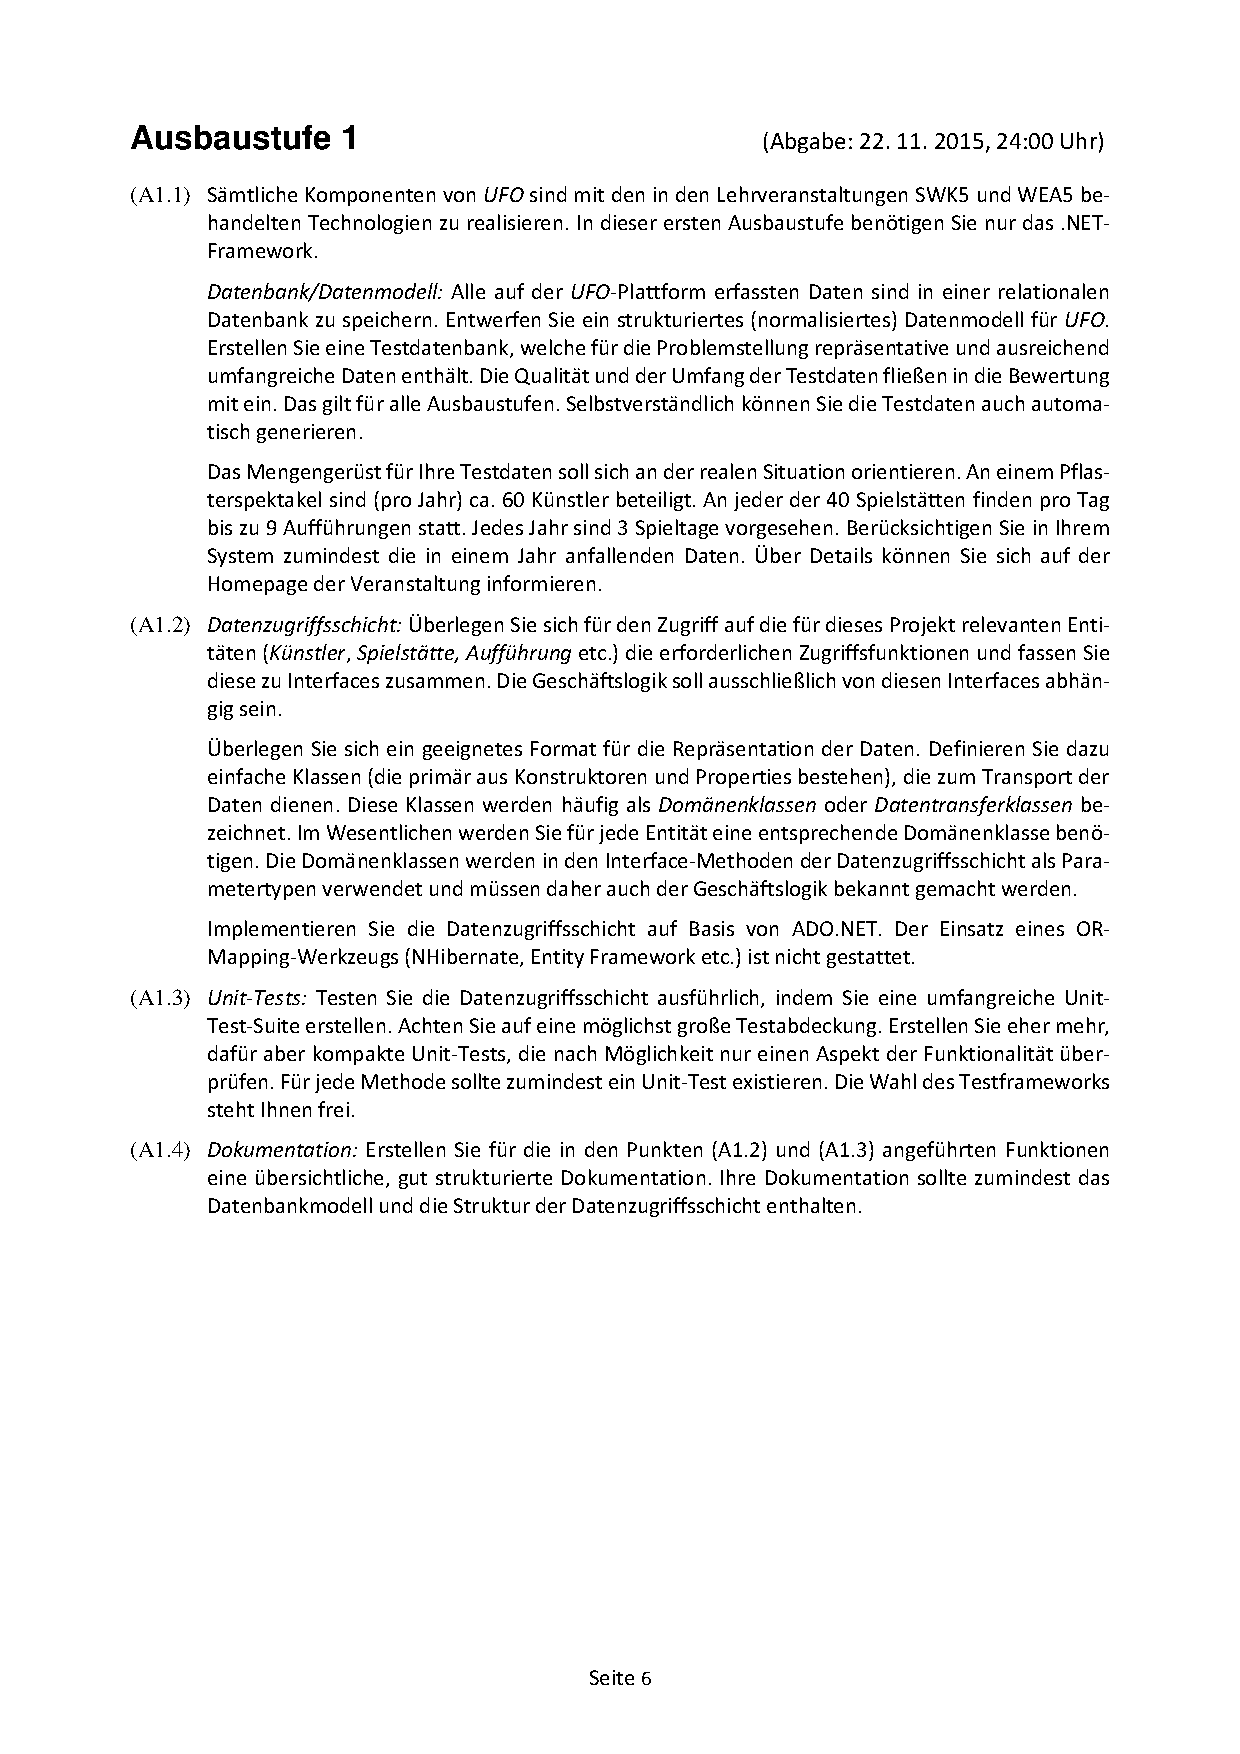
\includepdf[scale=1, pages={1}, angle=0]{./specs/Projekt-SWK5-WEA5-VZ-Ausbaustufe1.pdf}

    % sections
    \begin{section}{Framework Tools}

\subsection{PostSharp}
PostSharp (Aspekt orientierte Programmierung):
Dieses Tool wird verwendet, um eigene Aspekte bzw. Attribute schreiben zu können. Konkret wurde es für das Exception Handling in der DAL Schnittstelle verwendet. Das Attribut „DaoExceptionhandlerAttribute“ fängt eine auftretende Exception (z.B. bei einer Datenbank Abfrage) ab und wrappt diese in das generische DAOResponse Objekt. In weiterer Folge wird dieses Konzept noch näher erläutert. Nachfolgend wird beschrieben wie PostSharp in Visual Studio eingebunden werden kann. Für die Ausführung wird eine Free-Lizenz verwendet.

\subsubsection{Installation}
Unter folgendem Link kann PostSharp runtergeladen werden.\newline
\url{https://www.postsharp.net/download}

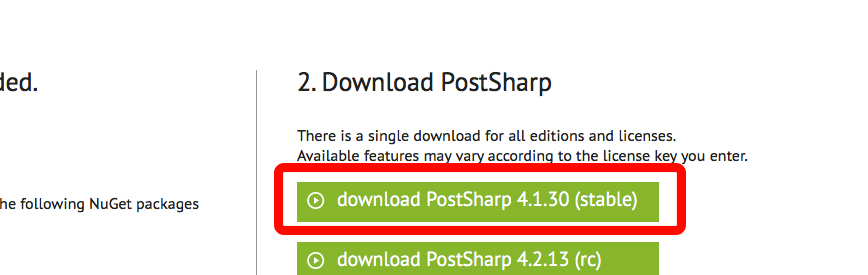
\includegraphics[angle=0, scale=0.45]{./img/postsharp1.jpg}
\FloatBarrier

\subsubsection{Registrierung / Account anlegen}
Um PostSharp im PostCompile Ablauf verwenden zu können, wird wie unten dargestellt, eine Freie Lizenzregistrierung benötigt.

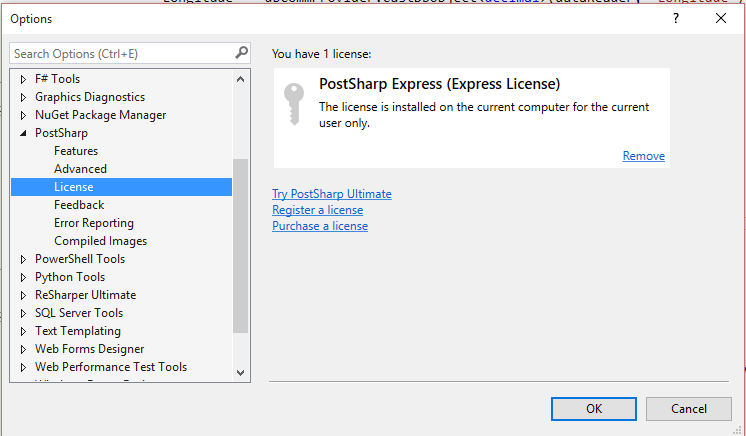
\includegraphics[angle=0, scale=0.45]{./img/postsharp3.jpg}
\FloatBarrier

		
\end{section}
    \newpage
		\begin{section}{Datenbankmodell}

\subsection{ER-Model}
Nach Analyse der Anforderungen, wurde das nachfolgende Domainmodell entworfen.
Zusätzlich zu den vorgegebenen Entitäten (user, artist, ...), werden noch zwei weitere benötigt: Location und Country.
Da es möglich ist, dass an einer Location (z.B. Landhaus, Hauptplatz...) mehrere Spielstätten (Venues) existieren, wird durch auslagern der Information in eine eigene Entität Datenredundanz vermieden.
\\

Für die konkrete Implementierung, wurde in Erwin das Schema entworfen per ForwardEngineering an eine MySQL Datenbank exportiert. Diese wird über phpMyAdmin verwaltet und die SQL-Scripte wurden nachträglich via Exportfunktionalität von MySQL generiert.
\\

Die Primärschlüssel (IDs) der Entitäten User, Location und Artist werden in der Datenbank per Auto-Incrementation automatisch nummeriert. \\

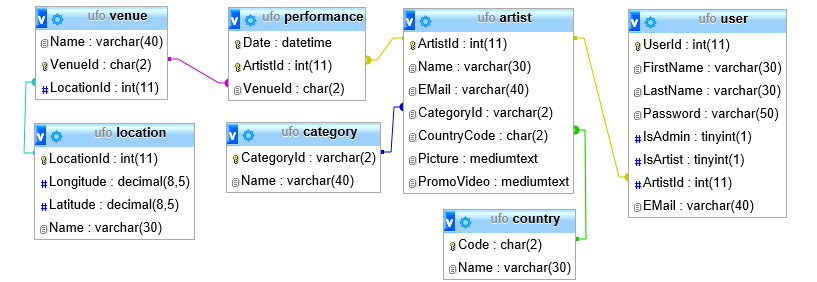
\includegraphics[angle=0, scale=0.45]{./img/databaseEntities.jpg}
\FloatBarrier

\subsection{Performance}
Um Aufführungen eindeutig abbilden zu können, wurde eine Primärschlüssel-Beziehung zwischen Artist und Venue in der Performance Entität erstellt. Diese bilden eine eindeutige Abbildung zu welcher Zeit und an welchem Ort ein Artist aufführt. Durch die Überprüfung der Zeit vor einfügen eines Datensatzes wird sichergestellt, dass ein Artist nicht eine Stunde vor bzw. nach seinem Auftritt wieder eingetragen werden kann.

\subsection{User}
Die Stammdatenverwaltung der User beinhaltet eine Referenz auf ein Artist Objekt, welches impliziert, dass der User nicht nur administrative Funktionalitäten beinhalten kann, sondern auch selbst als Artist funktionieren kann.
Wenn ein User auch ein Artist ist, wird das Flag IsArtist = 1 gesetzt.
Ein User kann auch als Admin deklariert werden mit IsAdmin = 1. Das heißt, er kann beide Eigenschaften beinhalten.
Diese Abbildung bildet die Basis für eine mögliche Erweiterung der Anwendung, wo sich User, die einem Artisten zugeordnet sind, einloggen können und Stammdaten wie Foto oder Promovideo selbst künftig ändern könnten.

\subsection{Artist}
Für Picture und PromoVideo werden Links in Form eines Strings in der Entität abgebildet. Die Pictures werden in einem BlobData Objekt abgeblidet, welches Meta-Informationen wie Name oder Pfad beinhaltet. Dieses Objekt ist serialisierbar und beinhaltet den Binärdatenstrom, welcher bis zum Client ins Frontend durchgetragen werden kann. \\

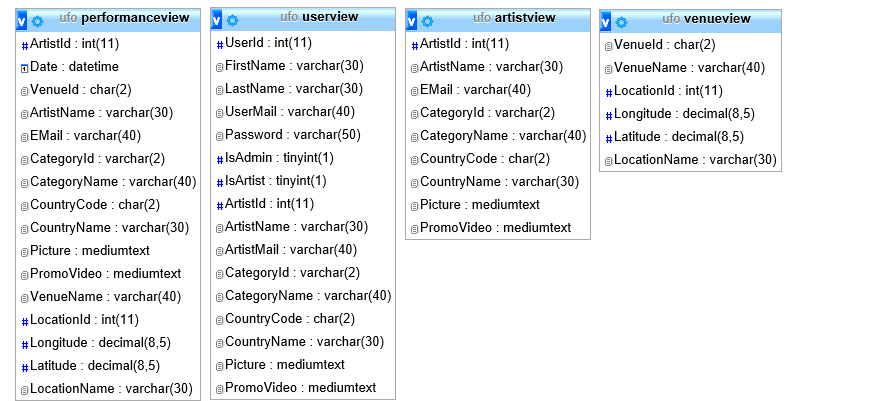
\includegraphics[angle=0, scale=0.45]{./img/databaseViews.jpg}
\FloatBarrier

\nPar

Des Weiteren werden vier Sichten erstellt: Performance-View, User-View, Artist-View und Venue-View. Dadurch können alle zusammenhängenden Daten mit einer Abfrage geladen werden und das verhindert Join-Statements im C\# Code.
Der wesentliche Vorteil besteht darin, dass gegebenenfalls alle benötigten Objekte mit einer Abfrage instanziiert werden können, wo ansonsten (wie im folgenden Beispiel) drei Anfragen an die Datenbank benötigt würden.

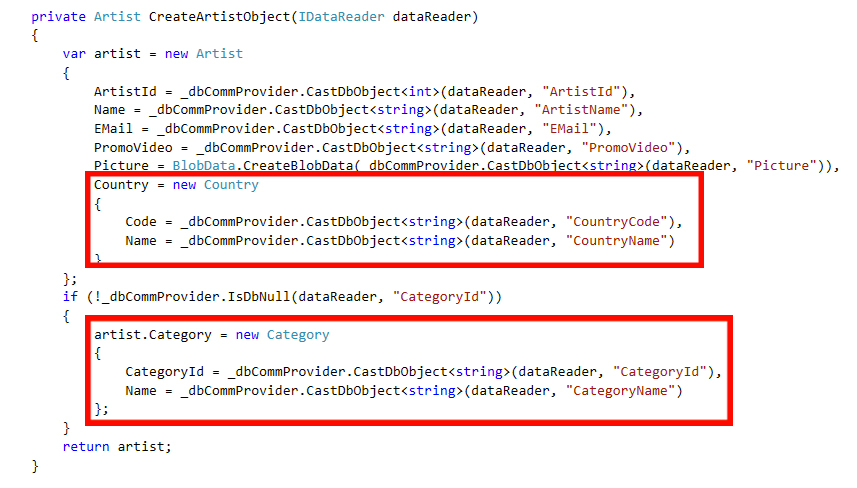
\includegraphics[angle=0, scale=0.45]{./img/viewcodesample.jpg}
\FloatBarrier

Zusätzlich um Nullwerte aus der Datenbank unterscheiden zu können und zum richtigen Datentyp mappen zu können, werden alle DataReader Zugriffe über die CastDbObject<T> Methode delegiert. Diese sorgt bei Nullwerten für den richtigen Standardwert.\\

\textbf{Die Daten in der Datenbank stammen von:} \\
User: \\ \url{http://convertcsv.com/generate-test-data.htm} \\
Country: \\ \url{http://blog.plsoucy.com/wp-content/uploads/2012/04/countries-20140629.csv} \\
Artist, Venue, Category, Location: \\ \url{http://www.pflasterspektakel.at/2015/de/1443.asp} (wurden manuell mit Excel angepasst) \\
Die jeweiligen SQL Scripten, wurden im Verzeichnis UFO.Database/sql bereitgestellt.


\end{section}
		\newpage
		\begin{section}{Implementation}

\subsection{UFO.Server}

\textbf{DalProviderFactories} \\
Erstellt zur Laufzeit eine DAO Factory, welche Methoden zur Erstellung von DAO-Instanzen beinhaltet. Die Klasse besteht aus einer statischen Methode, welche eine lose Koppelung zwischen Assemblies erstellt. Hierfür werden anstelle von internen Implementierungen die benötigten Daten aus der app.config Datei (XML) referenziert. Alle konkreten DAO Implementierungen beinhalten, welche von IDaoProviderFactory signiert werden. Wie intern die Instanziierung der DAOs gehandhabt wird obliegt der verwendeten Implementierung.

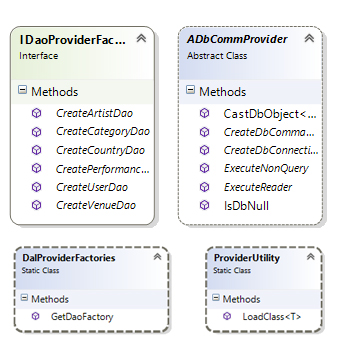
\includegraphics[angle=0, scale=0.45]{./img/DaoProviderFactory.jpg}
\FloatBarrier

\subsection{UFO.Server.Dal.Dummy}
Für die erste Implementierung wurde ein Dummy Assembly erstellt, welches von der IDaoProviderFactory ableitet und demonstrativ den Wechsel der Assemblies veranschaulichen soll. Es wurde jedoch nur ein Bruchteil der DAO Funktionalität implementiert und wird nur noch für Testzwecke verwendet.

\subsection{UFO.Server.Dal.MySQL}

Es werden die einzelnen DAOs instanziiert, diese stellen die benötigten Methoden zur Kommunikation (Connection, SELECT, INSERT, UPDATE, DELETE...) mit der Datenbank zu Verfügung.
Im UFO.Server.Dal.Common befindet sich eine abstrakte Klasse ADbCommProvider, welche die Basisklasse für eine gemeinsame Datenbankkommunikation darstellt. In diesem werden nur abstrakte Klassen wie DbConnection, DbCommand usw. (Klassen des .NET Frameworks) verwendet und des weiteren bietet diese abstrakte Methode, welche von den konkreten Technologien wie Beispielsweise die MySQL-Adaptoren implementiert werden können. \\

Das Basiskonzept der DAOs beruht auf ein gemeinsamen Responseobjekt, welches als Wrapper für das eigentliche Rückgabeobjekt dient. Dieses bietet zusätzliche Metainformationen und Funktionalitäten.
Es wurde nach dem Fluetinterface Modell nachempfunden. Das heißt, das Methoden wie OnSuccessful und OnFailure auch wiederum DAOResponse Objekte (also sich selbst) retournieren und diese per Chaining aufgerufen werden können. \\
Bsp.: \\

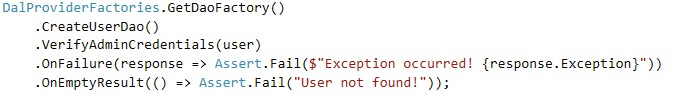
\includegraphics[angle=0, scale=0.75]{./img/snippet.jpg}
\FloatBarrier

\nPar

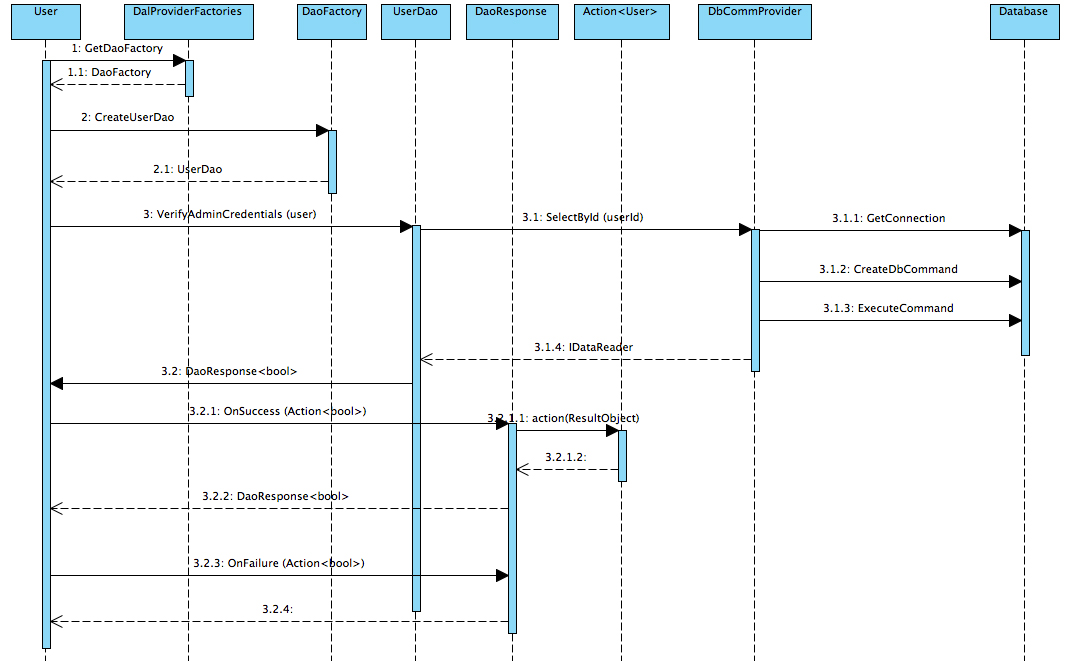
\includegraphics[angle=0, scale=0.45]{./img/SequenceDiagram.jpg}
\FloatBarrier

\nPar

Möglich ist diese Aufruffolge nur, weil keine der DAO Methoden eine Exception im Fehlerfall wirft.
Die Fehler werden durch das oben erwähnte Attribut (DaoExceptionHandlerAttribute) abgefangen und in ein DAOResponse Objekt gepackt und es wird sichergestellt, dass der Methoden-Kontrollfluss normal retourniert. \\
Die DAOResponses bestehen neben dem jeweiligen Datenobjekt, aus einen StatusCode (Successful, Failed, EmptyResult) gegebenenfalls auch eine Exception und einer Exception Message. \\
Der Vorteil dabei ist, dass alle Informationen (inkl. mögliche Fehler) in einem Objekt zusammengepackt werden und einfacher darauf reagiert werden kann. Die Exception werden an einer zentralen Stelle behandelt Anstelle von laufenden try-catch Blöcken.

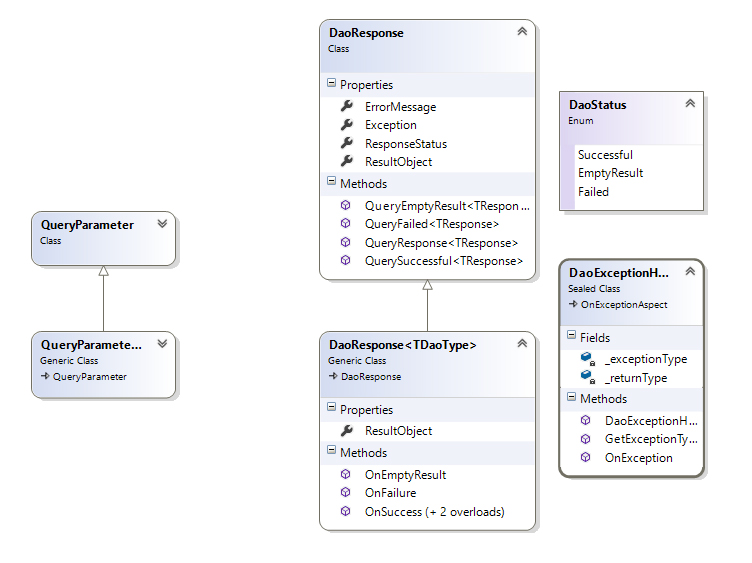
\includegraphics[angle=0, scale=0.45]{./img/DaoResponse.jpg}
\FloatBarrier

\subsection{UFO.Server.Dal.Common}
Beinhaltet die \textbf{Interfaces der einzelnen DAOs}. \\
Die Implementierung der DAOs wird nicht direkt vom ICommonDao Interface instanziiert, sondern es gibt für jedes DAO noch ein eigenes Interface, welches von ICommonDao erbt. \\

Es kann vorkomme, dass gewisse DAOs unterschiedliche Funktionalitäten benötigen können, welche nicht in einem gemeinsamen Basisinterface aggregiert werden können.
Ein konkretes Beispiel hierfür wäre die GetById Methoden, welche unterschiedliche Parameterdatentypen entgegennehmen. \\
Z.B.: Ist der Parameter für die CategoryId vom Typ „string“ wohingegen die LocationId vom Typ „Integer“ ist. Desweitern stehen dem Benutzer des Frameworks nur die Interfaces zur Verfügung und dieser kann nicht auf die konkreten Klassen zugreifen. \nPar
Die Methode SelectWhere<T> wird derzeit intern in der MySql Implementierung über die SelectAll Methode delegiert und verwendet den Lambda Ausdruck „Nur für in Memory Filterung“. Da jedoch eine Expression als Schnittstellen Definition zur Verfügung steht, kann diese in Zukunft zu einer nativen SQL Abfrage abgeändert werden, um somit eine Performance Steigerung zu erzielen. Für Testzwecke wurde auf Basis von SelectWhere auch die Extensionmethods erstellt. 

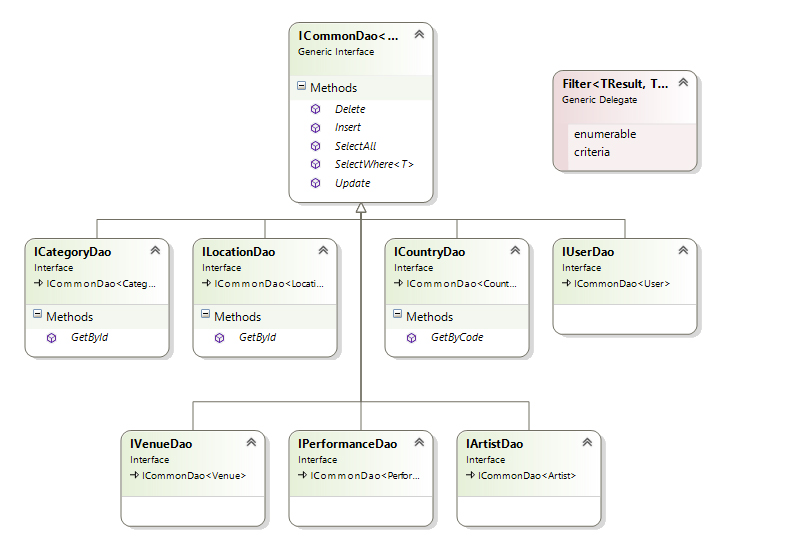
\includegraphics[angle=0, scale=0.45]{./img/DaoInterfaceClasses.jpg}
\FloatBarrier

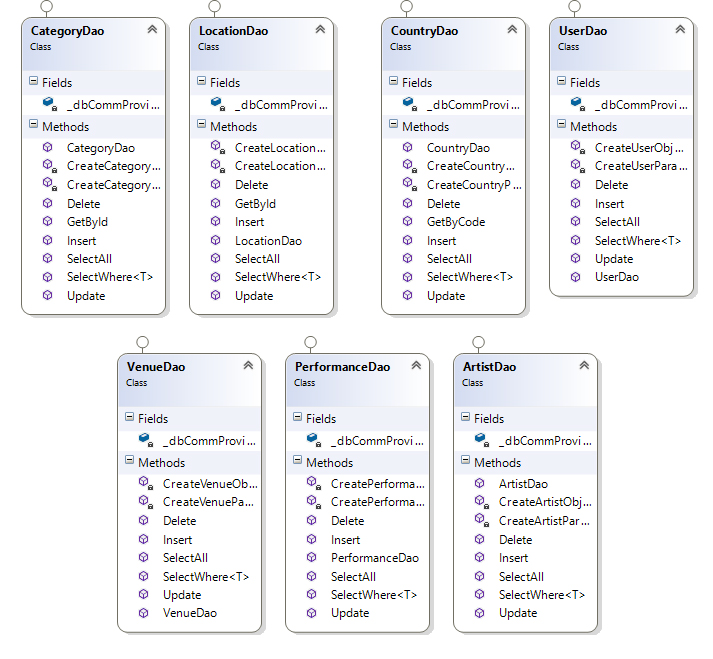
\includegraphics[angle=0, scale=0.45]{./img/DaoClasses.jpg}
\FloatBarrier

In manchen Fällen ist es Vorteilshaft, wenn zu den DAOs Erweiterungen (Extensions) implementiert werden.
So können Interfaces erweitert werden, ohne diese selbst zu verändern und Extensions sind einfach austauschbar bzw. lassen sich einfach wieder entfernen. Hier werden sie für Methoden verwendet, welche für die Testfälle nützlich sind, aber eventuell bei der nächsten Ausbaustufe des Projekts obsolet werden.


\subsection{UFO.Server.Dal.Domain}
Beinhaltet die Objekte zur Abbildung der Entitäten aus der Datenbank sowie die Klasse BlobData, welche in späterer Folge für die Abbildung von Mediendateien benötigt wird.

\nPar

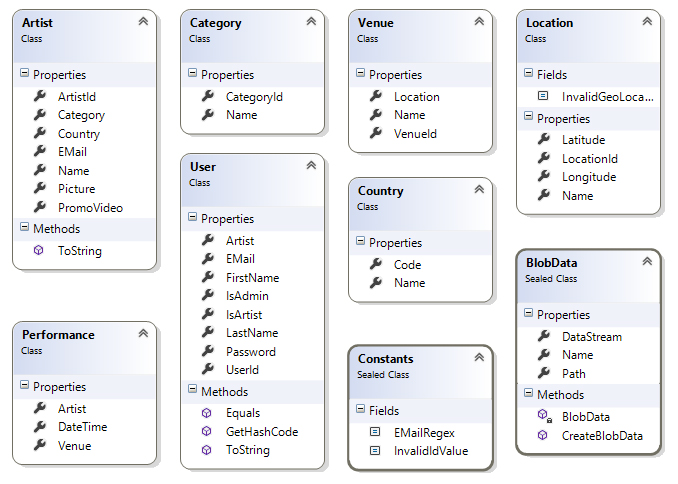
\includegraphics[angle=0, scale=0.45]{./img/ufoDomainClasses.jpg}
\FloatBarrier

\nPar

Außerdem wird die Klasse \textbf{Crypto} zur Verfügung gestellt. Welche für die Verschlüsselung von Passwörtern zuständig ist.
Diese Klasse beinhaltet zwei Methoden. Die eine Methode transformiert einen Klartext Stringwert in einen mit MD5 verschlüsselten Hashwert, welcher auch in die Datenbank gespeichert wird.
Die zweite Methode vergleicht den neu berechneten Hashcode mit dem aus der Datenbank.
Für diese Funktionalität werden Methoden aus dem .NET-Framework (System.Security.Cryptography) verwendet.



\end{section}
    
\end{document}